% \subsection{Stratified buffer vessel}
\subsubsection{Stratified buffer vessel}

This document describes the buffer vessel model that can be incorporated into the HAN dynamic house model. The buffer vessel model is the general model for a "stratified (layered) tank". The model for the buffer vessel is derived from the paper of Rakesh Sinha et al. \cite{sinha2020flexibility}. The model consists of a heating element, located outside of the buffer vessel, which can take water from the vessel and heat the water to a desired temperature.The hot water is then injected to the top of the buffer vessel. Hot water is is taken from the top of the buffer vessel on the demand side. Cooled water coming from the load is returned tot the bottom of the vessel. In this configuration, extensive convection in the tank, is avoided. 

\textbf{Model description}

A schematic description of the buffer vessel is shown below.

\begin{figure}[H]
	\centering
	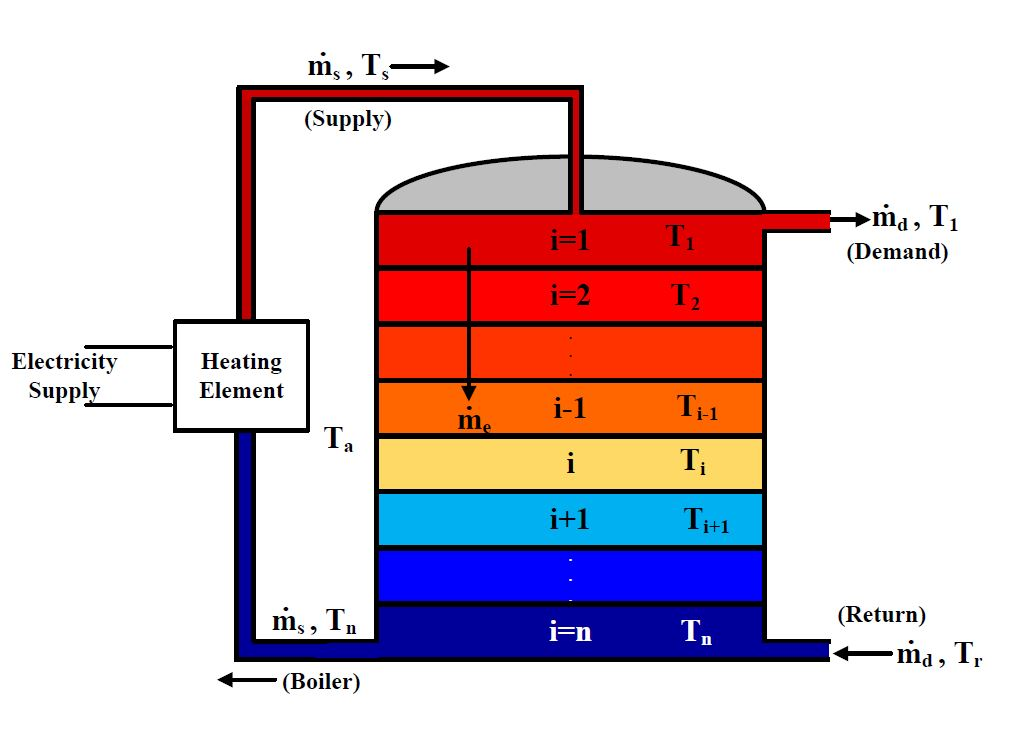
\includegraphics[width=0.8\columnwidth]{Figures/buffervessel_setup.JPG}
	\caption[Short title]{Buffer vessel representation}
\end{figure}

Due to the fact that the density of water decreases with temperature above 4 $\degC$, different temperature layers are created. In order to model this, the buffer vessel will be divided into $N$ different sections 

\textbf{Mathematical description}

\textbf{List of symbols:}

\begin{itemize}
	\item [$m$] {mass [kg]}
	\item [$\dot{m}$] {mass flow [kg/s]}
	\item [$C_w$] {Specific heat of water [J/kg]}
	\item [$T$] {Temperature [C]}
	\item [$U$] {Thermal transmittance [W/K]}
	\item [$A$] {Area [\(m^2\)]}
	\item [$\lambda$] {Heat conductivity [W/mK]}
\end{itemize}

\begin{equation}
	\begin{aligned}
		\label{eq:Buffer vessel layers}
	    mC_w \dfrac{dT_1}{dt} &=
	    \dot{m_s}C_w(T_s - T_1) + \dot{m_e}C_w(T_1 - T_2)*sgn(\dot{-m_e}) - UA_s(T_1 - T_a) - \frac{A_q\lambda_w}{z}(T_1-T_2) \\
	    mC_w \dfrac{dT_i}{dt} &= \\
	    & \dot{m_e}C_w(T_{i-1} - T_{i})*sgn(\dot{m_e}) + \dot{m_e}C_w(T_{i} - T_{i+1})*sgn(\dot{-m_e}) - UA_s(T_i - T_a) + \frac{A_q\lambda_w}{z}(T_{i-1} + T_{i+1} - 2T_i) \\
   	    mC_w \dfrac{dT_n}{dt} &= 
   	    \dot{m_d}C_w(T_r - T_n) + \dot{m_e}C_w(T_{n-1} - T_n)*sgn(\dot{m_e}) - UA_s(T_n + T_a) + \frac{A_q\lambda_w}{z}(T_{n-1}-T_n)		
	\end{aligned}
\end{equation}

\textbf{Validation}

To check to model from the paper, the following parameters are used:

\begin{figure}[h]
	\centering
	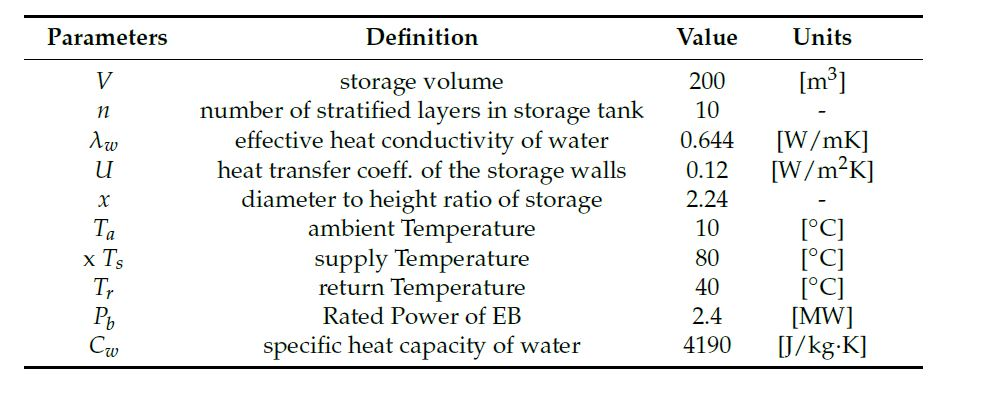
\includegraphics[width=0.6\columnwidth]{Figures/parameters_paper.JPG}
	\caption[Short title]{Buffer vessel parameters}
\end{figure}

This results in the following graph:

\begin{figure}[H]
	\centering
	\subfloat[\centering paper results]{{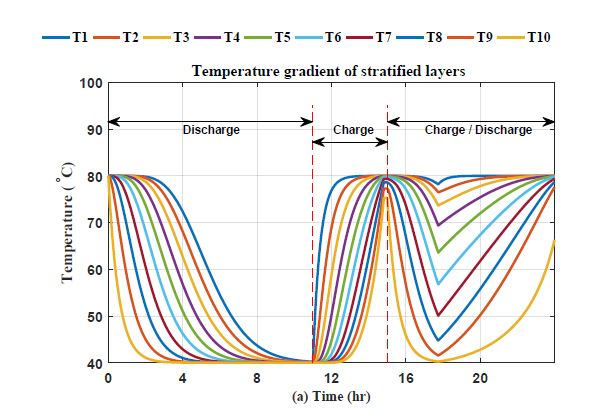
\includegraphics[width=0.5\columnwidth]{Figures/paper_results.jpg} }}
	\qquad
	\subfloat[\centering Python results]{{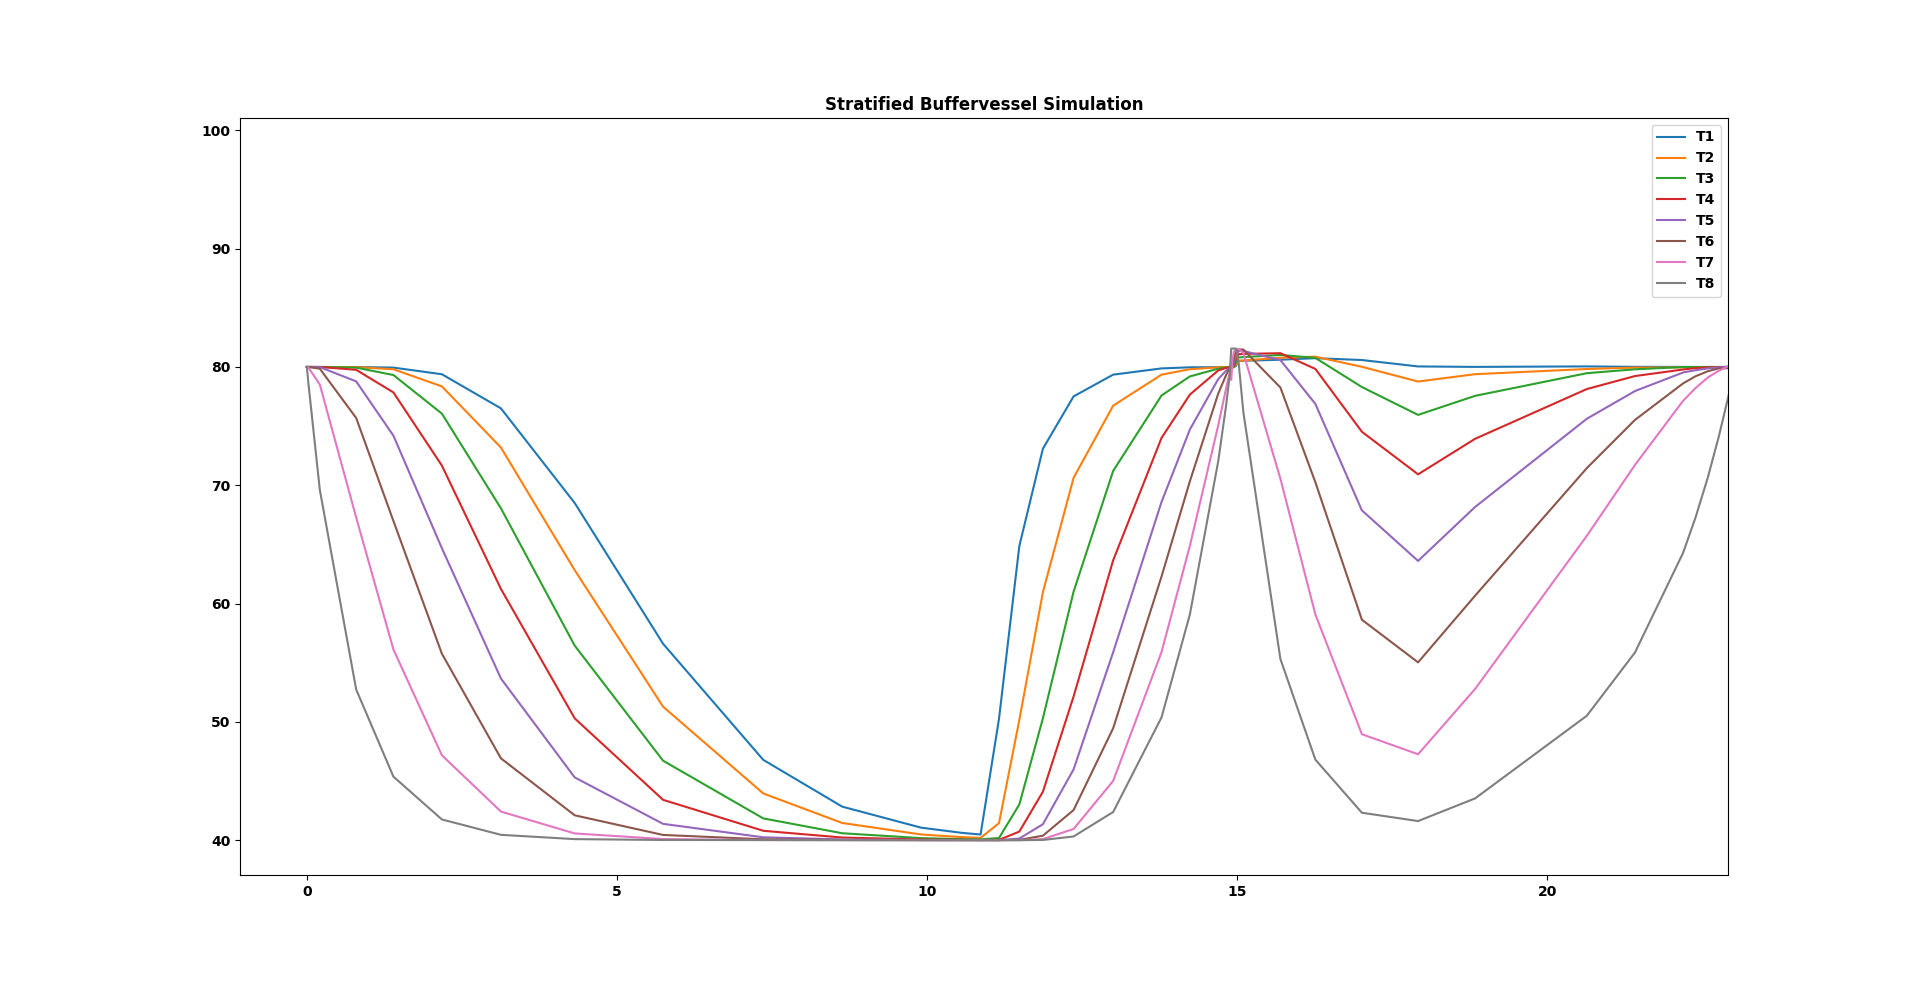
\includegraphics[width=0.5\columnwidth]{Figures/Python_validation_graph_buffervessel.png} }}
	\caption{Comparison between paper and python model}
	\label{fig:Comparison}
\end{figure}

\textbf{Matrix representation}

The differential equations [\ref{eq:buffer}] can be rewritten as:

{\color{teal}
	\begin{equation}
		\begin{aligned}
			C_{top}\frac{dT_{top}}{dt} &= \frac{-1}{R_{mid, top}} (T_{top}-T_{mid}) + \max(F_{rad}-F_{HP}, 0) \cdot (T_{mid} - T_{top}) \\
			&+ F_{HP} \cdot (T_{HP,out} - T_{top})
			\\ \\
			C_{mid}\frac{dT_{mid}}{dt} &= \frac{1}{R_{mid, top}} (T_{top}-T_{mid}) + \frac{-1}{R_{bot, mid}}(T_{mid}-T_{bot}) \\
			& + \max(F_{HP}-F_{rad}, 0) \cdot (T_{top} - T_{mid}) + \max(F_{rad}-F_{HP}, 0)  \cdot (T_{mid} - T_{bot}) 
			\\ \\
			C_{bot}\frac{dT_{bot}}{dt} &= \frac{1}{R_{bot, mid}} (T_{mid}-T_{bot}) + \max(F_{HP} - F_{rad}, 0) \cdot (T_{mid} - T_{bot})\\
			& + F_{rad} \cdot (T_{return} - T_{bot}) 
		\end{aligned}
	\end{equation}
}

These differential equations can be written in matrix notation as previously, but a \emph{convection} matrix $\mathbf{F}$ is added:

\begin{subequations}
	\label{eq:matnot}
	\begin{align}
		\mathbf{C} \cdot \boldsymbol{\dot{\theta}} + \mathbf{K} \cdot \boldsymbol{\theta} + \mathbf{F} \cdot \boldsymbol{\theta}= \mathbf{\dot{q}}
	\end{align}
\end{subequations}

with:

\begin{equation}
	\mathbf{C} \cdot \boldsymbol{\dot{\theta}} =
	\begin{bmatrix}
		C_{top} & 0 & 0 \\
		0 &  C_{mid} & 0 \\
		0 & 0 & C_{bot} \\
	\end{bmatrix}
	\cdot
	\begin{bmatrix}
		\frac{dT_{top}}{dt} \\
		\frac{dT_{mid}}{dt} \\
		\frac{dT_{bot}}{dt}
	\end{bmatrix}
\end{equation}

\begin{equation}
	\mathbf{K} \cdot \boldsymbol{\theta} =
	\begin{bmatrix}
		\frac{1}{R_{mid,top}} & \frac{-1}{R_{mid,top}} & 0\\
		\frac{-1}{R_{mid,top}} &  \frac{1}{R_{mid, top}} + \frac{1}{R_{bot,mid}} & \frac{-1}{R_{bot,mid}}\\
		0 &  \frac{-1}{R_{bot, mid}} & \frac{1}{R_{bot,mid}}
	\end{bmatrix}
	\cdot
	\begin{bmatrix}
		T_{top} \\
		T_{mid} \\
		T_{bot}
	\end{bmatrix}
\end{equation}

\begin{equation}
	\mathbf{F} \cdot \boldsymbol{\theta} =
	\begin{bmatrix}
		F_{HP,out} + F_{rad} & F_{rad} & 0 \\
		F_{rad} &  0  & F_{rad} \\
		0 &  F_{rad} & F_{HP} + F_{rad}
	\end{bmatrix}
	\cdot
	\begin{bmatrix}
		T_{top} \\
		T_{mid} \\
		T_{bot}
	\end{bmatrix}
\end{equation}

\begin{equation}
	\mathbf{\dot{q}} =
	\begin{bmatrix}
		\frac{1}{R_{air, amb}} \cdot T_{amb} + \dot{Q}_{heat, air} \\
		0
	\end{bmatrix}
\end{equation}


F1: [0 1 2 0]

F2: [2 1 0 2]

\begin{equation}
	\mathbf{DF_{F1}} = 
	\begin{bmatrix}
		0 & 1 &-1  \\
		-1 & 0 & 1  \\
		1 &-1 & 0  \\
	\end{bmatrix}
	\label{eq:DFflow1}
\end{equation}

\begin{equation}
	\mathbf{DF_{F2}} = 
	\begin{bmatrix}
		0 &-1 & 1  \\
		1 & 0 &-1  \\
		-1 & 1 & 0  \\
	\end{bmatrix}
	\label{eq:DFflow1}
\end{equation}

In each time step, when the flow sizes have been determined by the control algorithms, each directed-flow-matrix is multiplied by its respected flow size in [$\frac{\text{m}^3}{\text{s}}$]. All resulting matrices can then be added together. Assuming a flow of size $f_1$ and $f_2$ for the flows $F1$ and $F2$, respectively we now get the matrix $\mathbf{SF}$:
\begin{equation}
	\mathbf{SF} = f_1 \cdot \mathbf{DF_{F1}} + f_2 \cdot \mathbf{DF_{F2}} = 
	\begin{bmatrix}
		0     & \dot{f_1}-\dot{f_2} & \dot{f_2}-\dot{f_1} \\
		\dot{ f_2}-\dot{f_1}  & 0       & \dot{f_1}-\dot{f_2} \\
		\dot{f_1}-\dot{f_2}  & \dot{f_2}-\dot{f_1} & 0       
	\end{bmatrix}
	\label{eq:addbufferflows}
\end{equation}

The heat transfer induced by the flows is only in the direction of the water flow. The correct elements are obtained by taking the $\text{min}(\mathbf{SF},0)$, here we mean for each element in $\mathbf{SF}$ we take the minimum of the respective element and 0. Thus, in the case $f_1>f_2$ the matrix $\mathbf{SF}$ will become:
\begin{equation}
	\text{min}(\mathbf{SF},0) =  \begin{bmatrix}
		0     & \dot{f_1}-\dot{f_2} & 0 \\
		0     & 0       & \dot{f_1}-\dot{f_2} \\
		\dot{f_1}-\dot{f_2}  & 0       & 0     
	\end{bmatrix}
	\label{eq:minSFzero}
\end{equation}

Now, the diagonal elements can be computed. The diagonal elements are equal to minus the sum of the off-diagonal elements in its respective row. For the matrix given in equation \ref{eq:minSFzero} this results in the flow matrix $\mathbf{F}$:
\begin{equation}
	\mathbf{F} =  \begin{bmatrix}
		-(\dot{f_1}-\dot{f_2})   & \dot{f_1}-\dot{f_2} & 0 \\
		0     & -(\dot{f_1}-\dot{f_2})       & \dot{f_1}-\dot{f_2} \\
		\dot{f_1}-\dot{f_2}  & 0       & -(\dot{f_1}-\dot{f_2})     
	\end{bmatrix}
	\label{eq:flowmatrix}
\end{equation}

Finally, we need to multiply the resulting flow matrix with the density ($\rho_{w}$) and the specific heat ($c_{w}$), in order to obtain the heat transferred by the water due to the water flows. The resulting matrix can be added to the K matrix as given in equation \ref{eq:CKq_buffer}.

\begin{equation}
	\begin{aligned}
		\dot{f} = v_{pump} \cdot A_{pipe} \qquad & \left[ \frac{m}{s} \cdot m^2 = \frac{m^3}{s}\right] \\
		\dot{f} \cdot \rho_w \cdot c_w \quad \text{has the dimension} \qquad & \left[ \frac{m^3}{s} \cdot m^2 \cdot\frac{kg}{m^3} \cdot \frac{J}{kg \cdot K} = \frac{J}{K \cdot s} = \frac{W}{K}\right]
	\end{aligned}
\end{equation}


\usetikzlibrary{matrix,decorations.pathreplacing}
\pgfkeys{tikz/mymatrixenv/.style={decoration=brace,every left delimiter/.style={xshift=4pt},every right delimiter/.style={xshift=-4pt}}}
\pgfkeys{tikz/mymatrix/.style={matrix of math nodes,left delimiter=[,right delimiter={]},inner sep=1pt,row sep=0em,column sep=0em,nodes={inner sep=6pt}}}

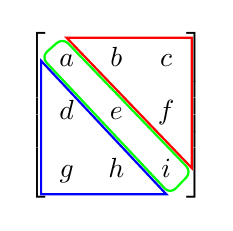
\begin{tikzpicture}[baseline=0cm,mymatrixenv]
	\matrix [mymatrix,text width=0.6em,align=center] (m)  
	{
		a & b & c \\ 
		d & e & f \\
		g & h & i \\
	};
	\pgfmathsetmacro{\offset}{0.5mm}
	\draw [thick,blue] (m-1-1.west) |- (m-3-3.south) -- cycle;
	\draw [thick,red] (m-1-1.north) -| (m-3-3.east) -- cycle;
	\draw [thick,green,rounded corners=1mm] ([yshift=\offset]m-1-1.west) -- ([xshift=-\offset]m-1-1.north) -- ([yshift=-\offset]m-3-3.east) -- ([xshift=\offset]m-3-3.south) -- cycle;
\end{tikzpicture}

\lstinputlisting[label=lst:stratified, linerange={178-216}, 
caption={StratifiedBufferNew class}] 
{../../housemodel/sourcesink/buffervessels/stratified.py}
